%%%%%%%%%%%%%%%%%%%%%%%%%%%%%%%%%%%%%%%%%
% University/School Laboratory Report
% LaTeX Template
% Version 3.1 (25/3/14)
%
% This template has been downloaded from:
% http://www.LaTeXTemplates.com
%
% Original author:
% Linux and Unix Users Group at Virginia Tech Wiki 
% (https://vtluug.org/wiki/Example_LaTeX_chem_lab_report)
%
% License:
% CC BY-NC-SA 3.0 (http://creativecommons.org/licenses/by-nc-sa/3.0/)
%
%%%%%%%%%%%%%%%%%%%%%%%%%%%%%%%%%%%%%%%%%

%----------------------------------------------------------------------------------------
%	PACKAGES AND DOCUMENT CONFIGURATIONS
%----------------------------------------------------------------------------------------

\documentclass{article}

\usepackage[version=3]{mhchem} % Package for chemical equation typesetting
%\usepackage{siunitx} % Provides the \SI{}{} and \si{} command for typesetting SI units
\usepackage{graphicx} % Required for the inclusion of images
\usepackage{natbib} % Required to change bibliography style to APA
\usepackage{amsmath} % Required for some math elements 
\usepackage{hyperref}
 \usepackage{pdflscape}
\usepackage[a4paper,margin=0.5in]{geometry}
\setlength\parindent{0pt} % Removes all indentation from paragraphs

\renewcommand{\labelenumi}{\alph{enumi}.} % Make numbering in the enumerate environment by letter rather than number (e.g. section 6)

%\usepackage{times} % Uncomment to use the Times New Roman font

%----------------------------------------------------------------------------------------
%	DOCUMENT INFORMATION
%----------------------------------------------------------------------------------------

\title{Gate Detection} % Title

\author{Philipp \textsc{Duernay}} % Author name

\date{\today} % Date for the report

\begin{document}
\maketitle
% If you wish to include an abstract, uncomment the lines below
% \begin{abstract}
% Abstract text
% \end{abstract}

%----------------------------------------------------------------------------------------
%	SECTION 1
%----------------------------------------------------------------------------------------

\section{Recap}
In the last meeting from 06.06.2018 several next steps were defined:
\begin{itemize}
	\item Finish two stage approach
	\item Study effect of fast architectures (mobilenet, shufflenet, wide-residual net)
\end{itemize}


\section{Fast architectures}

Last time I mentioned that there are fast architectures but that those are not implemented in darknet, which makes them difficult to use. However, there is one structure which can be used and those are the so called bottlenecks. The principle is displayed in \autoref{fig:bottleneck}. \autoref{tab:bottleneck} shows how the layer can save computations.

\begin{table}[htbp]
	\caption{Inference Time Bottleneck on JeVois}
	\begin{center}
		\begin{tabular}{|r|r|r|}
			\hline
			\multicolumn{1}{|l|}{\textbf{n\_filters (input vol 13x13x64)}} & \multicolumn{1}{l|}{\textbf{Standard Conv}} & \multicolumn{1}{l|}{\textbf{Bottleneck 0.5}} \\ \hline
			64 & 2.3 & 2 \\ \hline
			128 & 4.09 & 2.87 \\ \hline
			256 & 7.48 & 5.41 \\ \hline
		\end{tabular}
	\end{center}
	\label{tab:bottleneck}
\end{table}

\begin{table}[htbp]
	\caption{Inference Time Strides vs Pooling on JeVois}
	\begin{center}
		\begin{tabular}{|l|r|r|}
			\hline
			\textbf{Input + Filter} & \multicolumn{1}{l|}{\textbf{(2,2) Strides}} & \multicolumn{1}{l|}{\textbf{(1,1) Stride + MaxPool}} \\ \hline
			\textit{kernel6x6} & \multicolumn{1}{l|}{} & \multicolumn{1}{l|}{} \\ \hline
			208x208 & 35.6 & 144.1 \\ \hline
			104x104 & 9.6 & 37 \\ \hline
			52x52 & 2.6 & 9.7 \\ \hline
			& \multicolumn{1}{l|}{} & \multicolumn{1}{l|}{} \\ \hline
			\textit{kernel3x3} & \multicolumn{1}{l|}{} & \multicolumn{1}{l|}{} \\ \hline
			208x208 & 15.6 & 70.13 \\ \hline
			104x104 & 3.8 & 17.9 \\ \hline
			52x52 & 1.14 & 4.22 \\ \hline
		\end{tabular}
	\end{center}
	\label{tab:strides}
\end{table}

Additionally, I experimented with larger strides to reduce the computations. This led to the different models displayed in \autoref{fig:}

\begin{figure}
	\begin{minipage}{0.45\textwidth}
	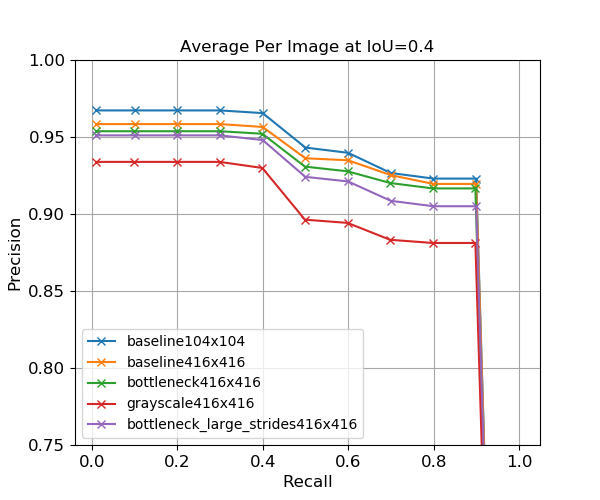
\includegraphics[width=\linewidth]{pr04}
	\end{minipage}
\begin{minipage}{0.45\textwidth}
	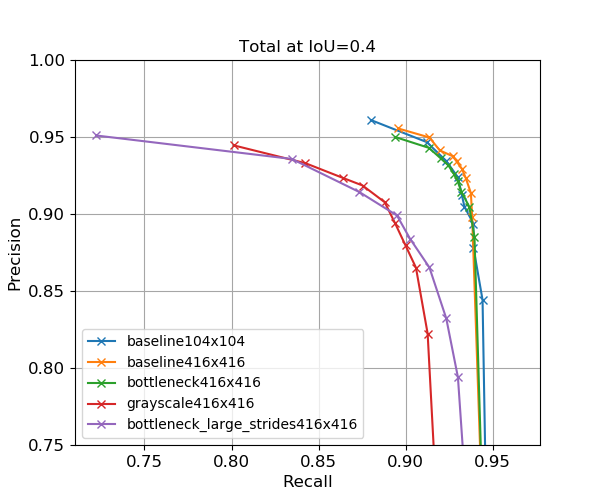
\includegraphics[width=\linewidth]{totalpr04}
\end{minipage}
\end{figure}

\begin{figure}
	\begin{minipage}{0.45\textwidth}
		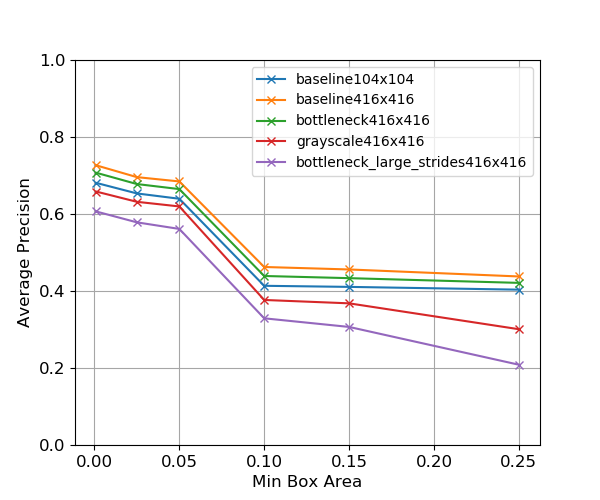
\includegraphics[width=\linewidth]{area}
	\end{minipage}
	\begin{minipage}{0.45\textwidth}
		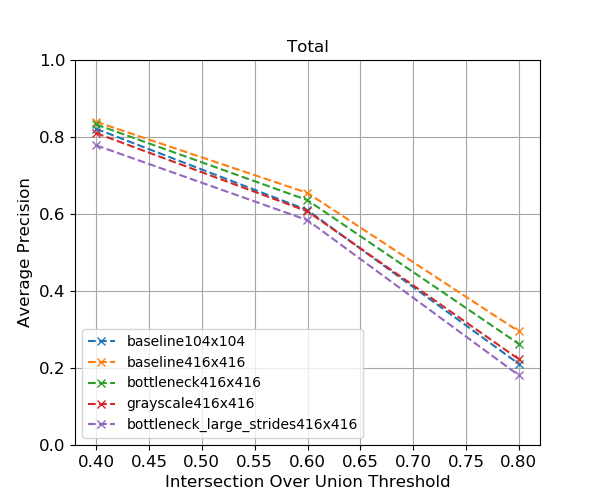
\includegraphics[width=\linewidth]{iou}
	\end{minipage}

\end{figure}

\begin{figure}
		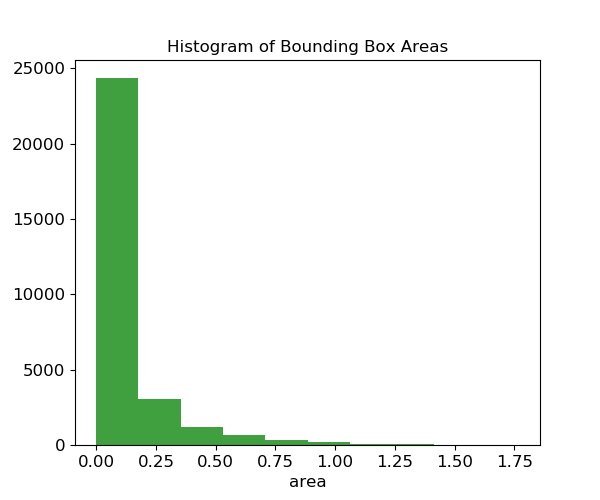
\includegraphics[width=0.5\linewidth]{hist_training}

\end{figure}

\newpage


\section{Conclusion}
\begin{itemize}
	\item Darknet enables us to use the GPU and run networks faster. However, we still can't process the image at full resolution.
	\item The two-stage approaches deliver a framework for our course-to-fine approach.
	\item In the first stage a 5-layer network seems to be enough to propose regions.
\end{itemize}

\section{Next Steps}
\begin{itemize}
	\item Write it all down.
	\item Finish implementation with two stage approach.
	\item Implement it in darknet.
	\item Investigate effect of depthwise separable convolutions on performance and speed.
	
\end{itemize}


\end{document}\grid
